\documentclass[twocolumn,a4paper]{article}

\usepackage{graphicx}

\begin{document}

\title{$\Gamma$-function}
\author{Wikipedia}
\maketitle

\begin{abstract}
    In mathematics, the gamma function (represented by $\Gamma$, the capital letter gamma from the Greek alphabet) is one commonly used extension of the factorial function to complex numbers.
\end{abstract}

\section{Introduction}

Text goes here

\begin{figure}[b]
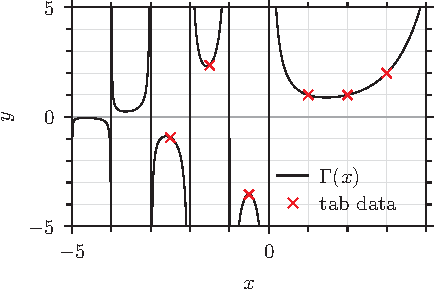
\includegraphics{gamma_pyx.pdf}
\end{figure}

%\begin{figure}[b]
%    \includegraphics{gamma_gnu.pdf}
%\end{figure}

\begin{equation} \label{my_label}
    \Gamma(z) = \int_0^\infty x^{z-1} e^{-x}\,dx, \ \qquad \Re(z) > 0\
\end{equation}

Here is an reference to an equation \ref{my_label}

\end{document}


